%%%%%%%%%%%%%%%%%%%%%%%%%%%%%%%%%%%%%%%%%%%%%%%%%%%%%%%%%%%%%%%%%%%%%%%%%%%%%%%%%%%%%%%%%%%%%%%%%%%%%%
%
%   Filename    : appendix_C.tex 
%
%   Description : This file is for including the Research Ethics Documents (delegated as Appendix C) 
%                 
%%%%%%%%%%%%%%%%%%%%%%%%%%%%%%%%%%%%%%%%%%%%%%%%%%%%%%%%%%%%%%%%%%%%%%%%%%%%%%%%%%%%%%%%%%%%%%%%%%%%%%

\chapter{Data Gathering Documentation}
\label{sec:appendixc}



% Save the file you want to include in PDF format.
% Uncomment the commant below specifying the correct appendix file. 
%\includepdf[pages=-, scale = 0.9, pagecommand={}, offset = -30 0]{appendixA.pdf}

This section of the paper presents the data gathering process, including spawning, dissection, sex identification, collection of linear measurements, and image capture from six different camera angles.


\begin{figure}[!htbp]
	\centering
	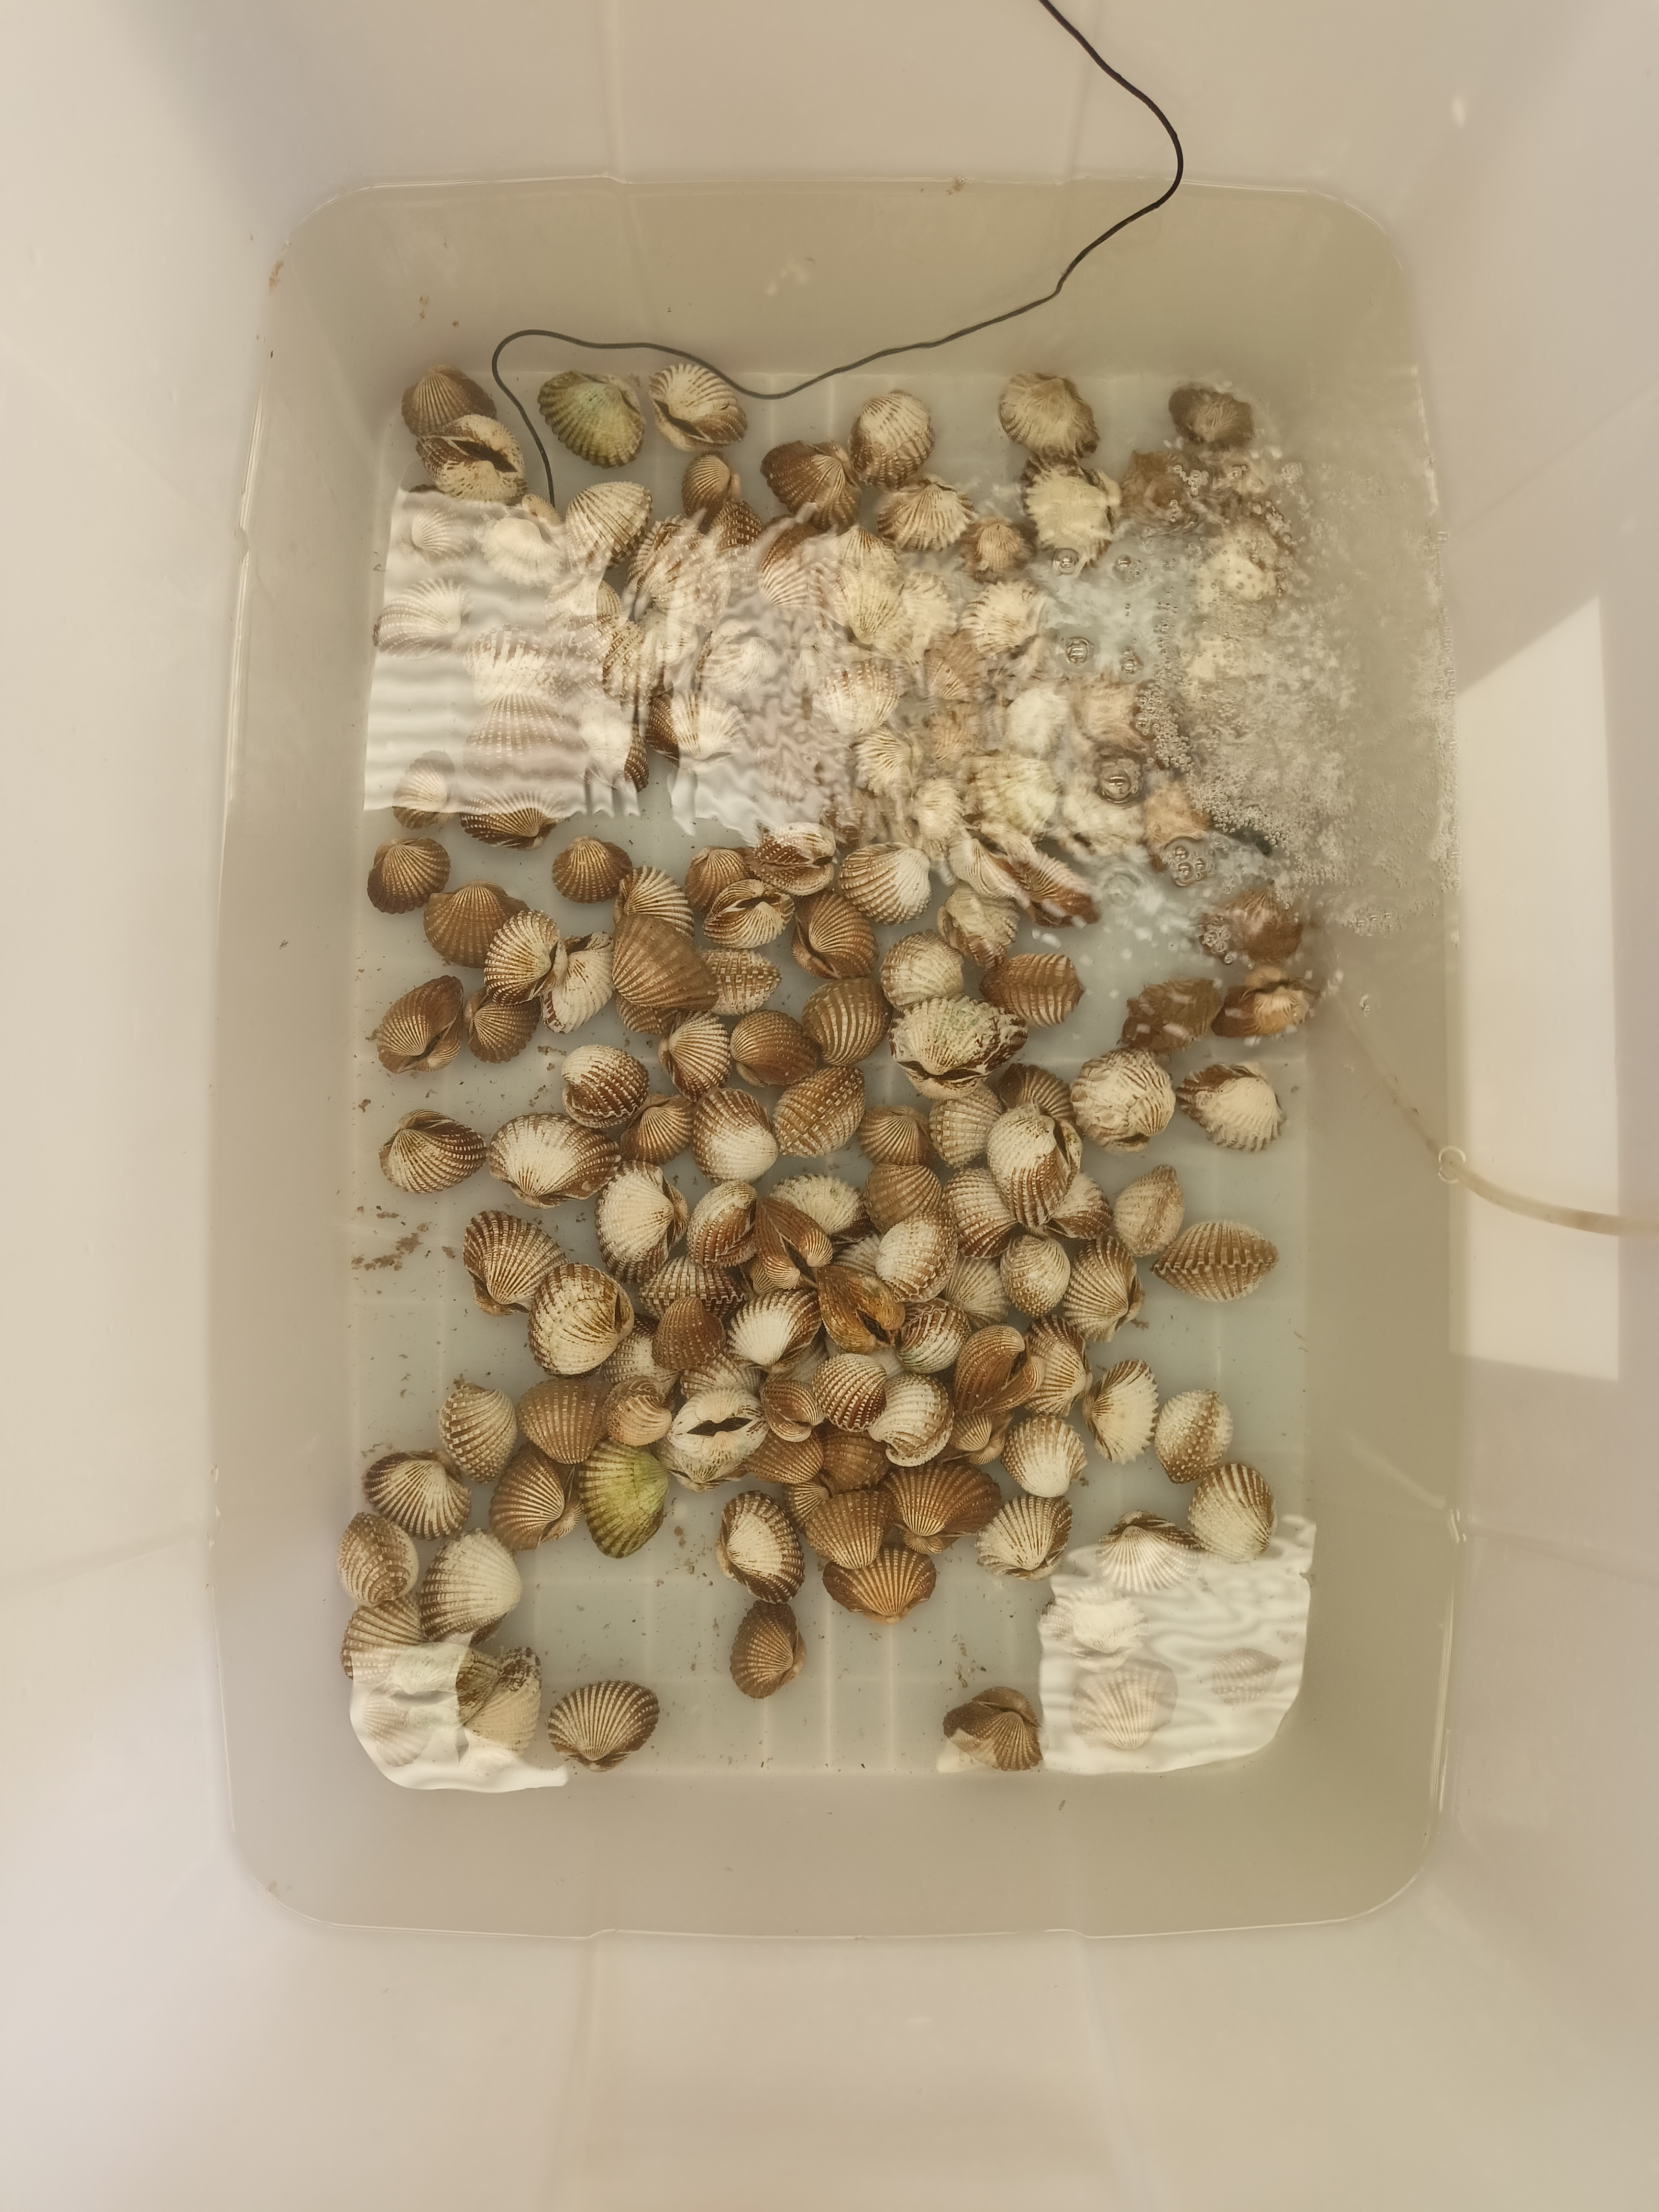
\includegraphics[width=0.4\textwidth, angle=90]{figures/spawning.jpg}
	\caption{Sex Identification Through Spawning of \textit{T. granosa}}
\end{figure}

\begin{figure}[!htbp]
	\centering
	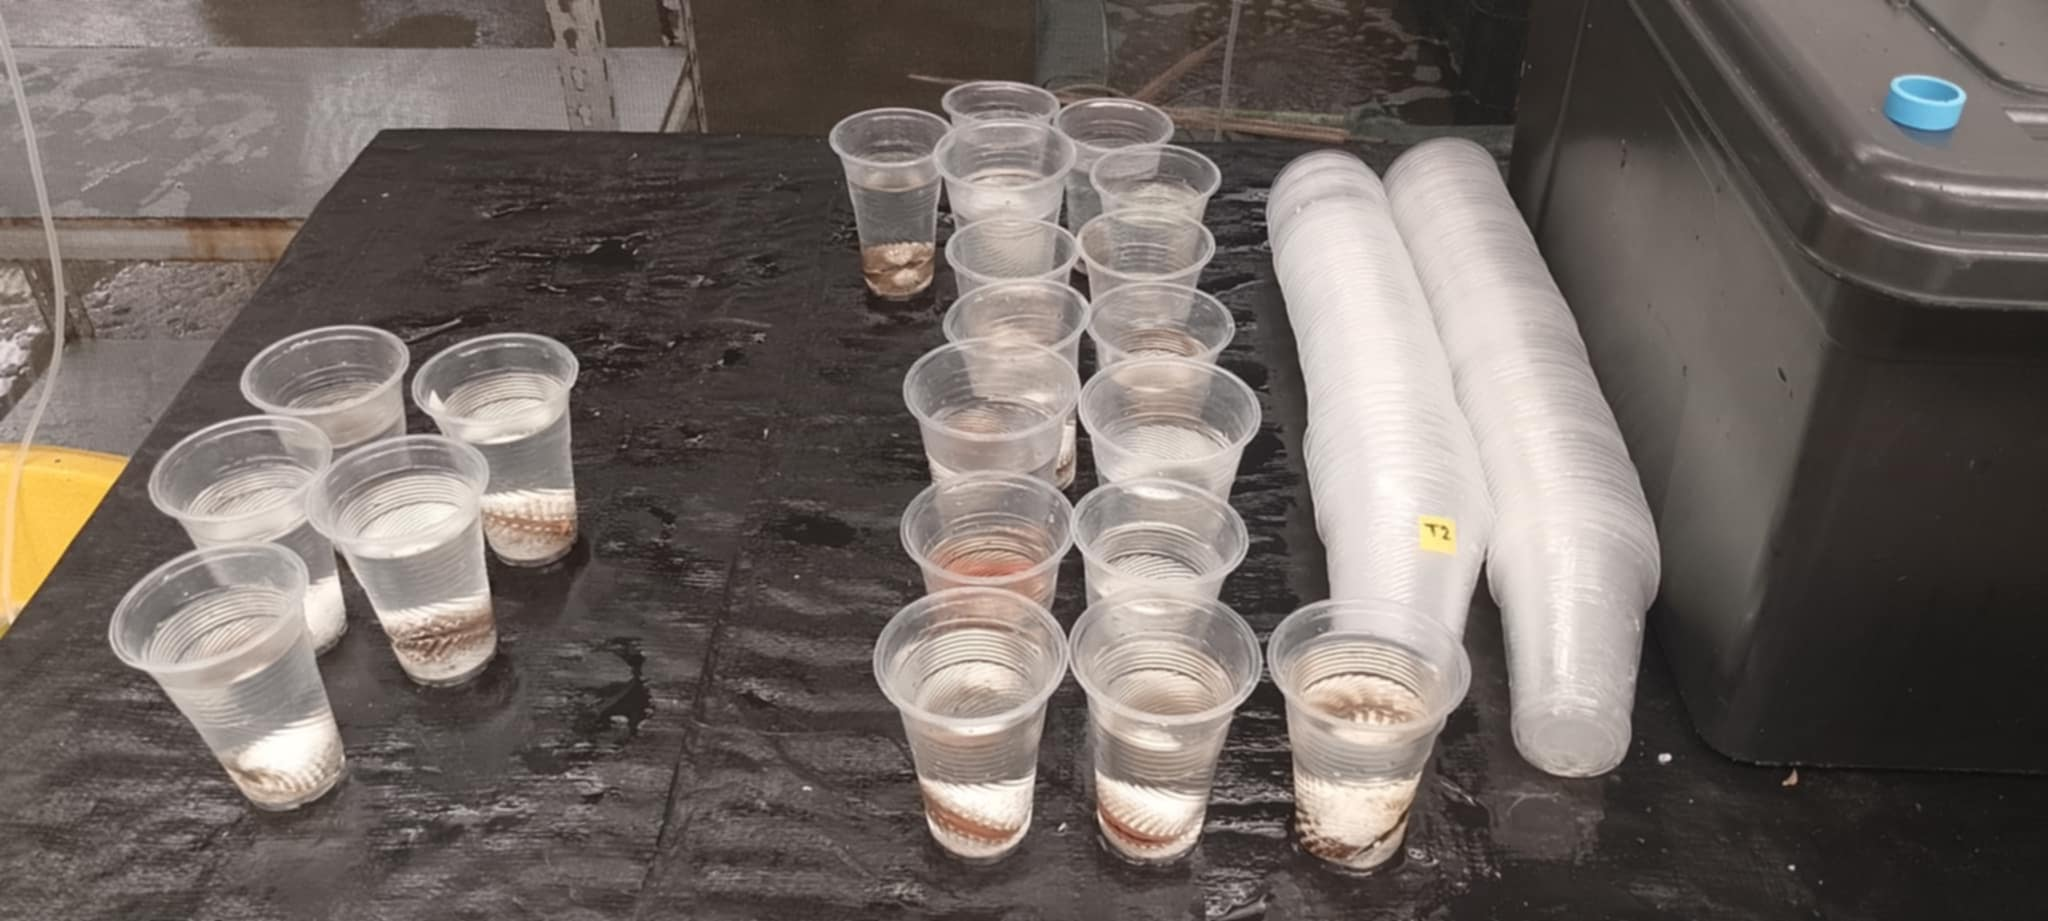
\includegraphics[width=0.55\textwidth]{figures/spawning_separated.jpg}
	\caption{Sex-Based Separation of \textit{T. granosa} Samples Post-Spawning}
\end{figure}

\begin{figure}[!htbp]
	\centering
	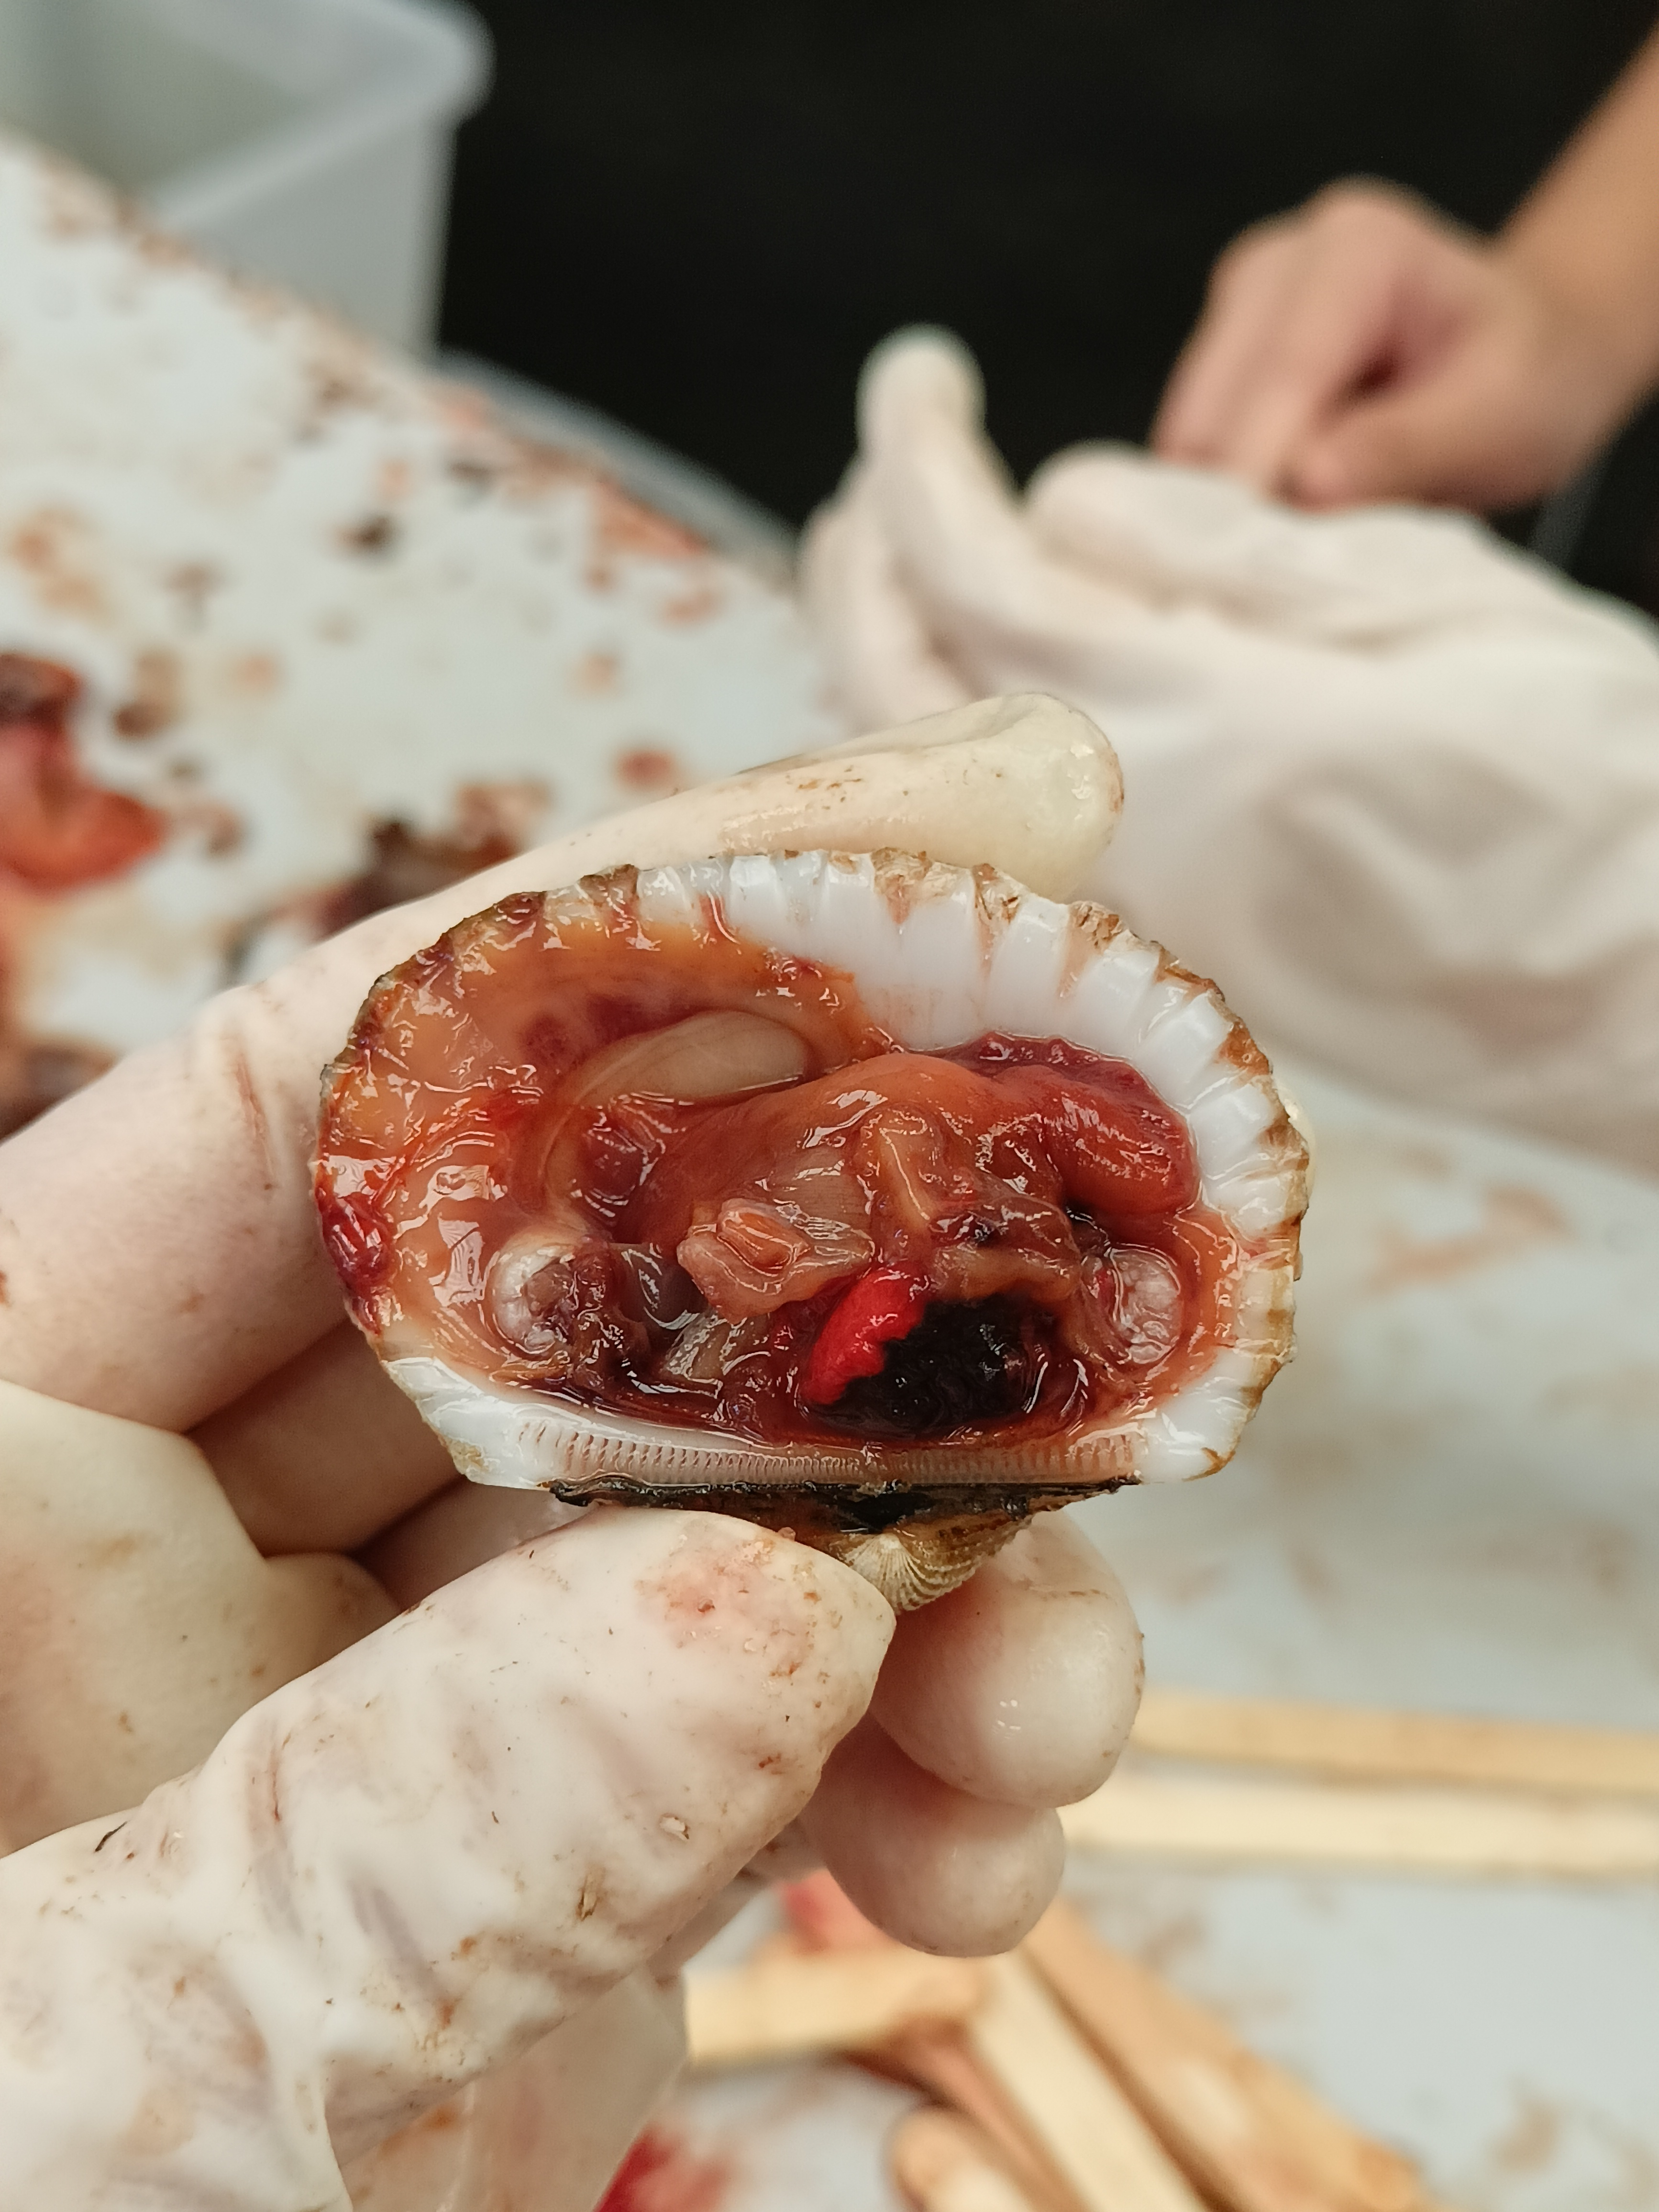
\includegraphics[width=0.4\textwidth, angle=90]{figures/dissecting_female.jpg}
	\caption{Sex Identified Female Through Dissection of \textit{T. granosa}}
\end{figure}

\begin{figure}[!htbp]
	\centering
	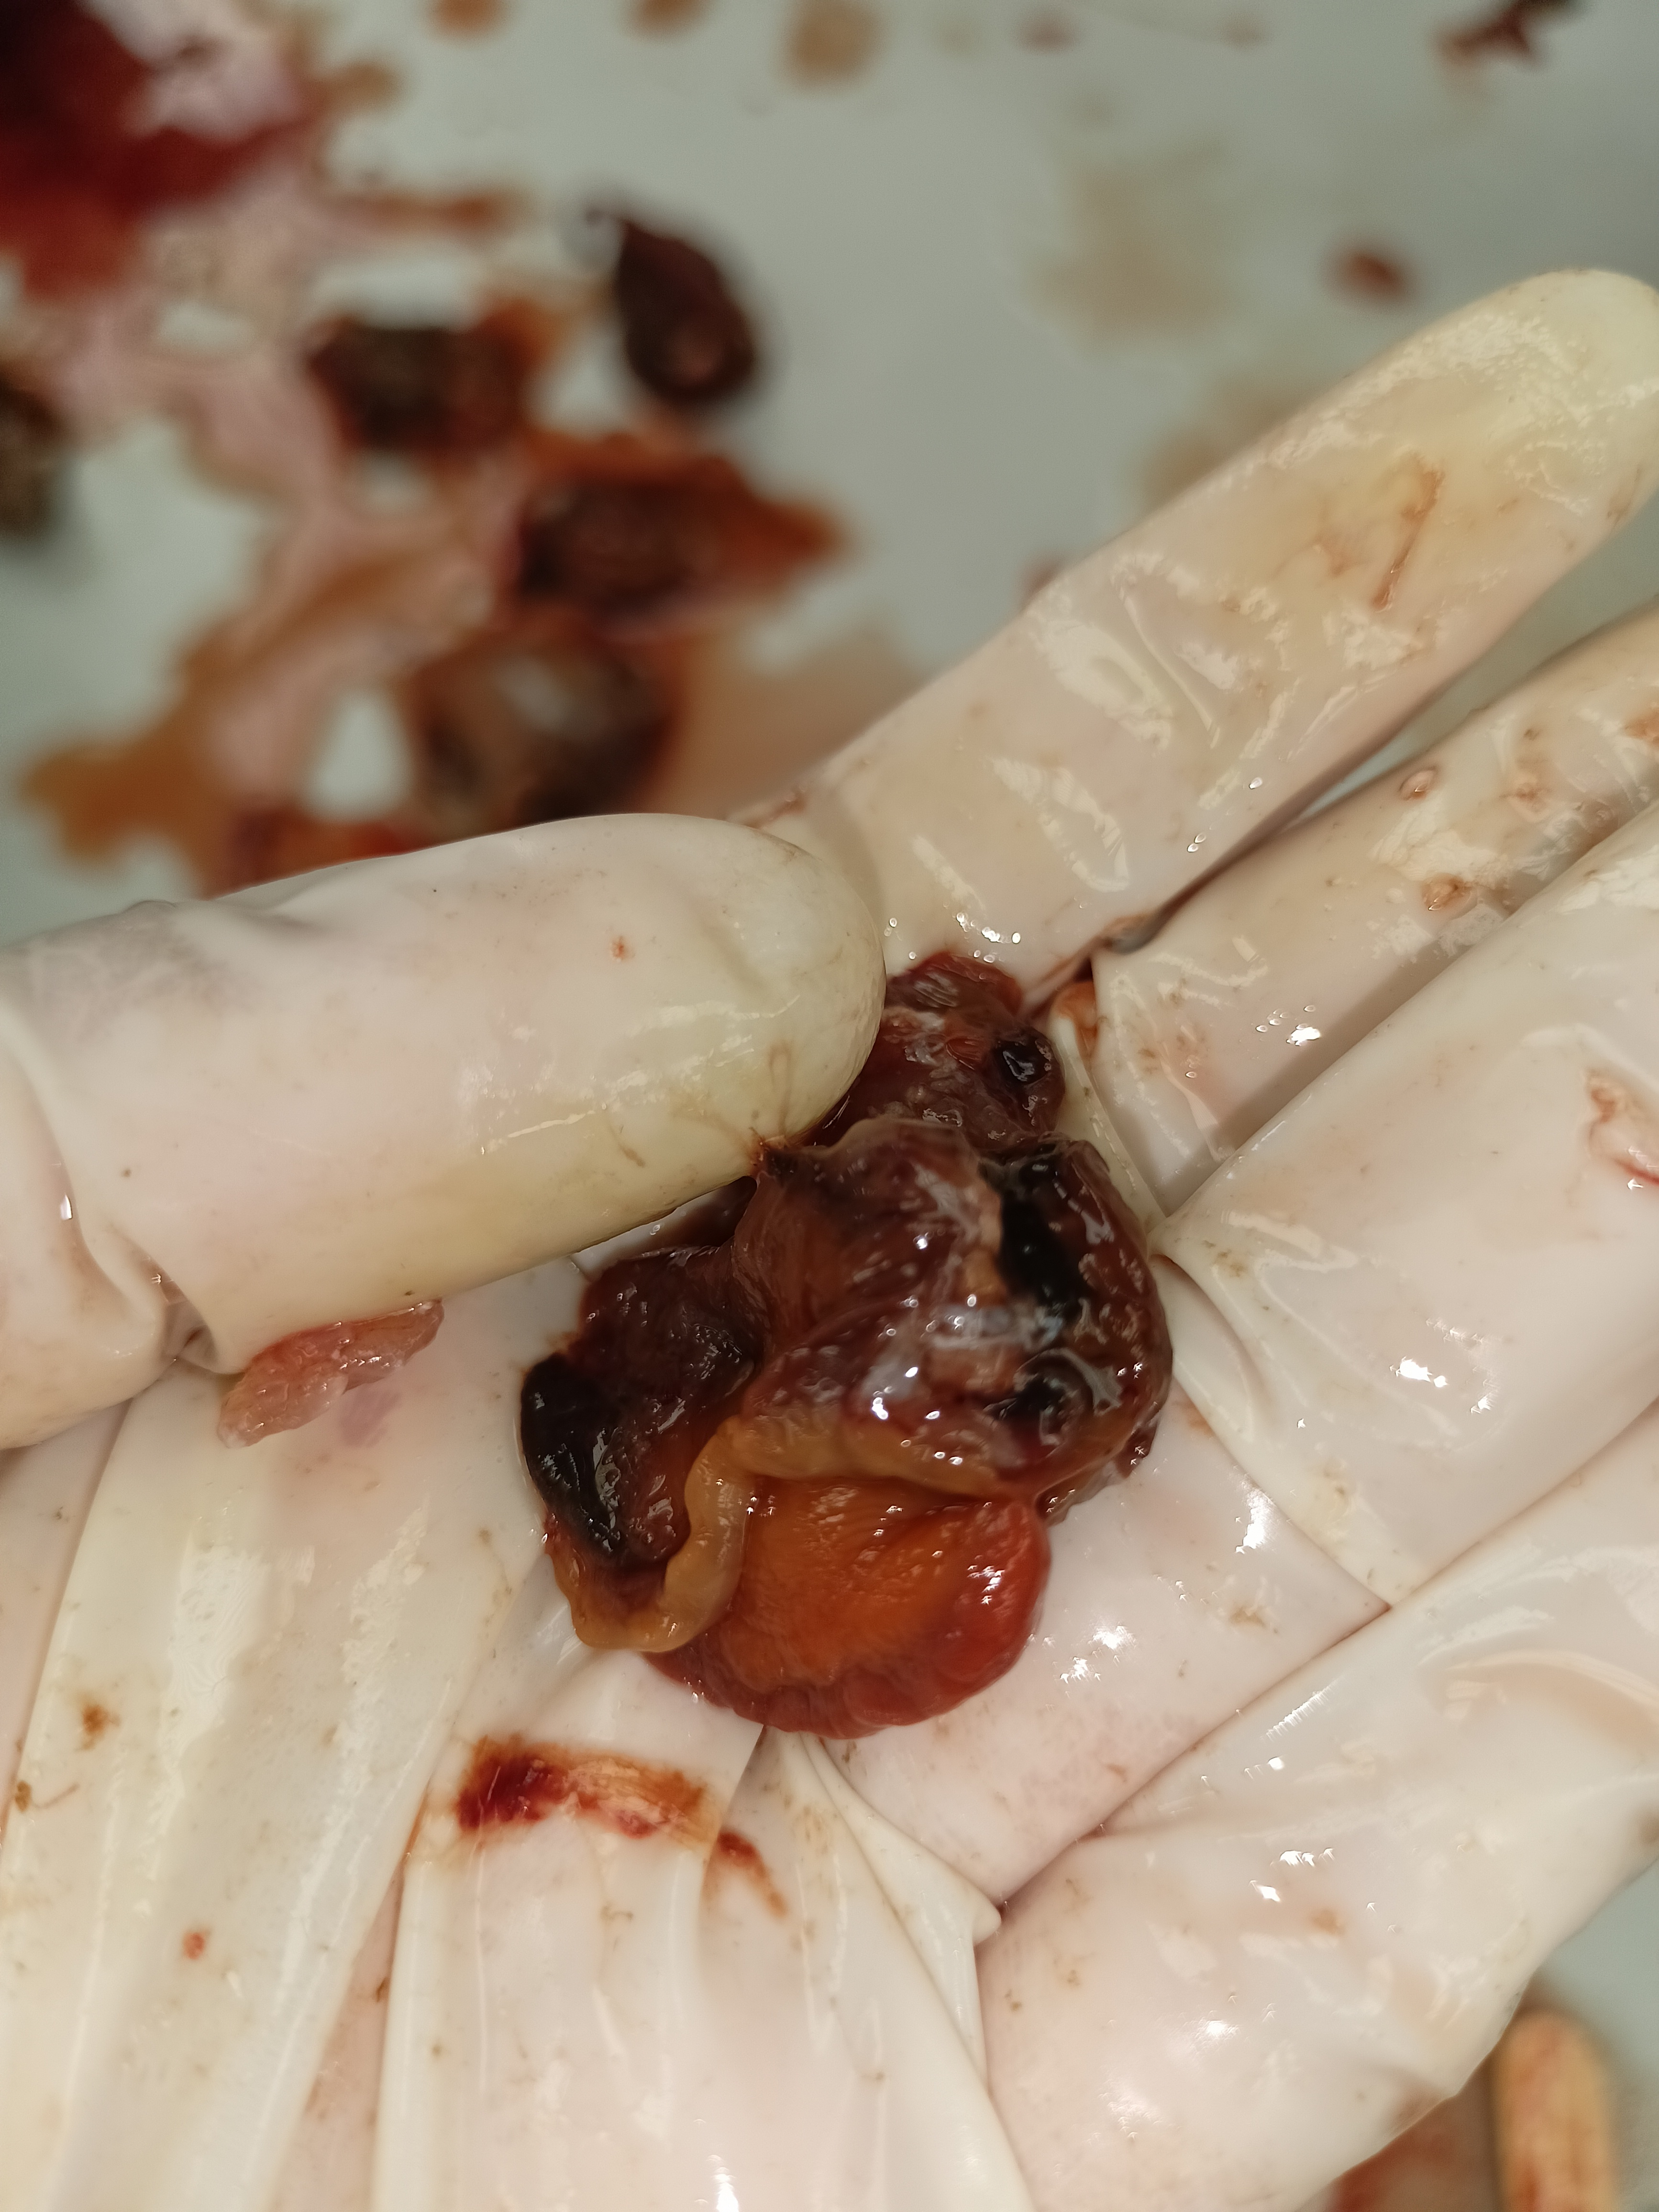
\includegraphics[width=0.4\textwidth, angle=90]{figures/dissecting male.jpg}
	\caption{Sex Identified Male Through Dissection of \textit{T. granosa}}
\end{figure}

\begin{figure}[!htbp]
	\centering
	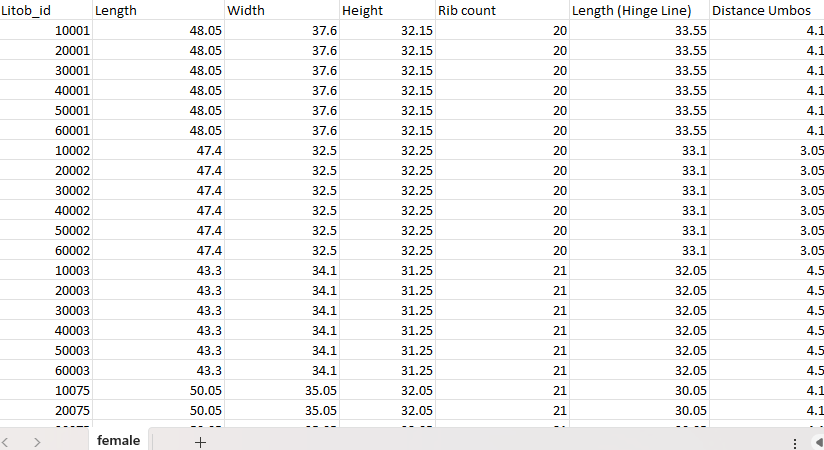
\includegraphics[width=0.6\textwidth]{figures/female_dataset.png}
	\caption{Linear Measurements of Female \textit{T. granosa}}
\end{figure}

\begin{figure}[!htbp]
	\centering
	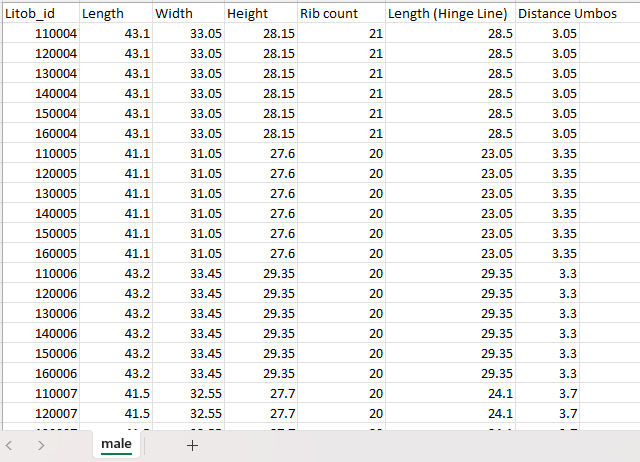
\includegraphics[width=0.6\textwidth]{figures/male_dataset.png}
	\caption{Linear Measurements of Male \textit{T. granosa}}
\end{figure}

\begin{figure}[!htbp]
	\centering
	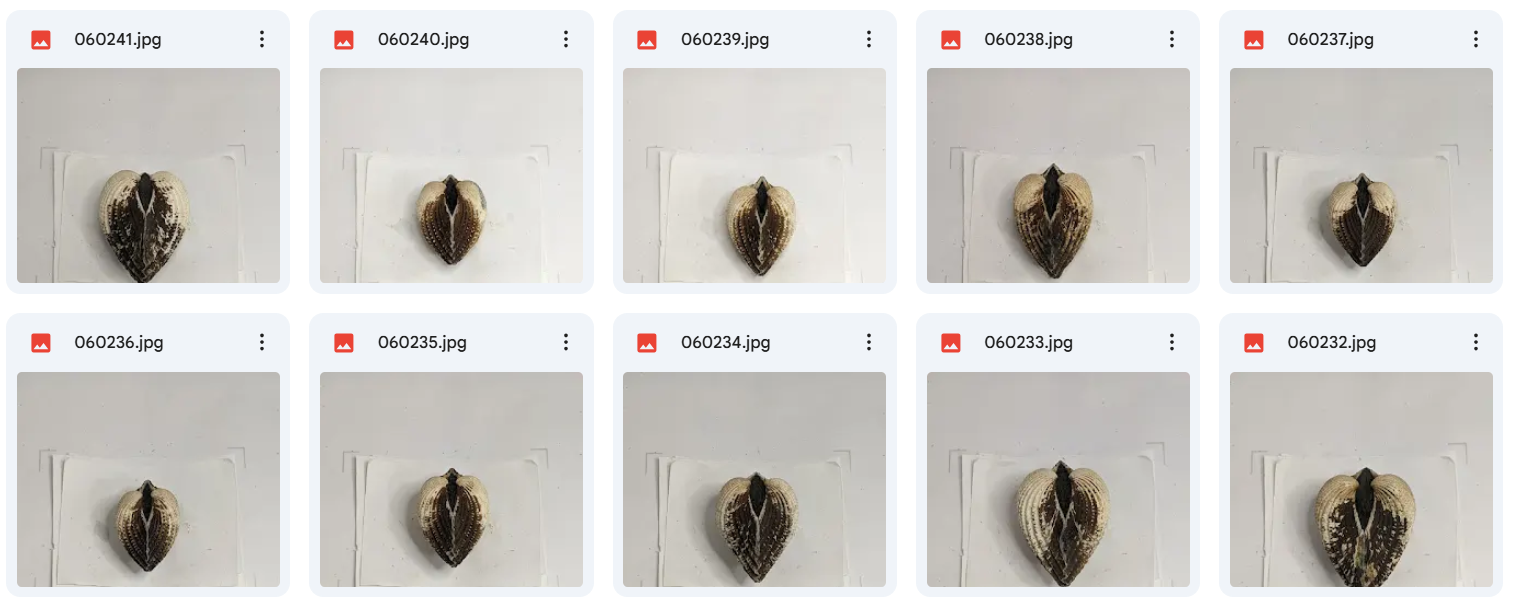
\includegraphics[width=0.8\textwidth]{figures/female_dataset(img).png}
	\caption{Captured Images of Female \textit{T. granosa}}
\end{figure}

\begin{figure}[!htbp]
	\centering
	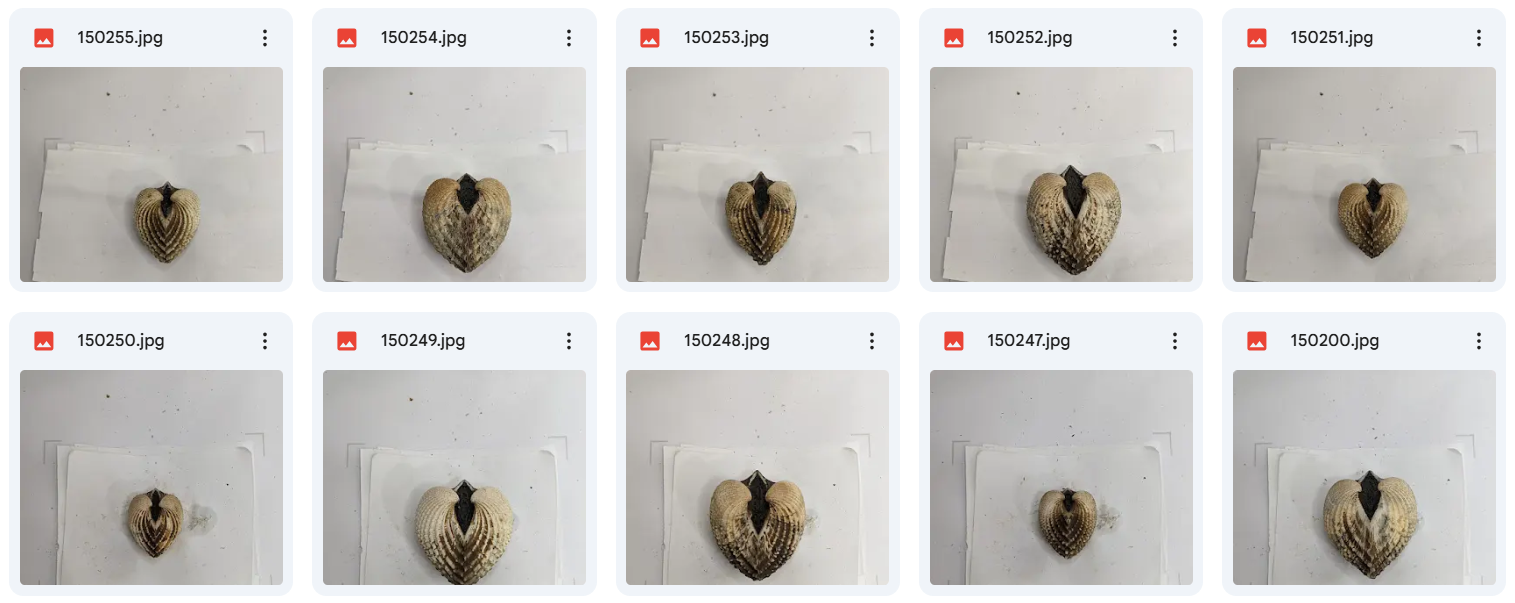
\includegraphics[width=0.8\textwidth]{figures/male_dataset(img).png}
	\caption{Captured Images of Male \textit{T. granosa}}
\end{figure}
